\documentclass[main.tex]{subfiles}
\begin{document}

\chapter{Random Variables and Distribution Functions}\label{ch:rastgele-degiskenler}

A probability space\index{probability space@probability space} is an abstract structure: $\Omega$ may consist of sequences of coin tosses, particle positions or stock price paths. In statistics, however, we work with \emph{numerical} summaries of these outcomes. A random variable\index{random variable@random variable} is a function that carries the abstract $\Omega$ into the real numbers while preserving the probability structure. In this chapter we show that the distribution of a random variable is completely determined by a single function, the CDF\index{distribution function cdf@distribution function (CDF)}; we study the characteristic properties of the CDF and the inverse transform method\index{inverse transform method@inverse transform method} that underlies random number generation.

\section{Definitions}

\begin{definition}[Borel $\sigma$-Algebra and Random Variable]\label{def:rd}
The smallest $\sigma$-algebra generated by all open intervals of $\R$ is called the Borel $\sigma$-algebra ($\B(\R)$). A function from a probability space\index{probability space@probability space} $(\Omega, \F, \P)$ to $(\R, \B(\R))$ such that $X^{-1}(B) \in \F$ for every $B \in \B(\R)$ is called a \emph{random variable\index{random variable@random variable}} (RV).
\end{definition}

\begin{remark}
$\B(\R)$ is also generated by the family $\{(-\infty,x]: x\in\R\}$. Hence, for $X$ to be a random variable it is \emph{sufficient} that $\{\omega: X(\omega)\le x\}\in\F$ for every $x\in\R$. (Idea of proof: the family $\{B : X^{-1}(B)\in\F\}$ is a $\sigma$-algebra containing the generating family.)
\end{remark}

\begin{definition}[Distribution]
If $X$ is an RV, the measure $\P_X$ defined by $\P_X(B)=\P(X^{-1}(B))=\P(X\in B)$, $B\in\B(\R)$, is called the \emph{distribution} (or law) of $X$. $(\R,\B(\R),\P_X)$ is a probability space in its own right. If $\P_X=\P_Y$, then $X$ and $Y$ are said to be \emph{identically distributed}, written $X\overset{d}{=}Y$.
\end{definition}

\begin{definition}[Distribution Function (CDF)]\index{distribution function cdf@distribution function (CDF)|textbf}
The cumulative distribution function of $X$, $F_X:\R\to[0,1]$, is defined by $F_X(x)=\P(X\le x)$.
\end{definition}

\begin{definition}[Discrete and Continuous Random Variables]
\begin{enumerate}
  \item $X$ is \emph{discrete} if it takes values in a countable set $\{x_1,x_2,\dots\}$; the function $p_X(x)=\P(X=x)$ is called the \emph{probability mass function} (pmf), and $F_X(x)=\sum_{x_i\le x}p_X(x_i)$.
  \item $X$ is \emph{(absolutely) continuous} if $F_X(x)=\int_{-\infty}^x f_X(t)\,dt$ for some non-negative integrable $f_X$; $f_X$ is called the \emph{probability density function} (pdf). At points where $f_X$ is continuous, $F_X'(x)=f_X(x)$.
\end{enumerate}
\end{definition}

\begin{definition}[Quantile (Generalised Inverse) Function]
For $u\in(0,1)$, the function $F^{-1}(u)=\inf\{x\in\R: F(x)\ge u\}$ is called the \emph{quantile function\index{quantile function@quantile function}} of $F$. If $F$ is continuous and strictly increasing, this is the ordinary inverse. $F^{-1}(1/2)$ is the median.
\end{definition}

\begin{definition}[Empirical Distribution Function]
For a sample $X_1,\dots,X_n$, the function
\[
\hat F_n(x)=\frac1n\sum_{i=1}^n \I\{X_i\le x\}
\]
is called the \emph{empirical distribution function\index{empirical distribution function@empirical distribution function}} (ECDF). For every fixed $x$, $n\hat F_n(x)\sim\text{Bin}(n,F(x))$.
\end{definition}

\section{Main Theorems and Proofs}

\begin{theorem}[Characteristic Properties of the CDF]\label{thm:cdf-ozellik}\index{distribution function cdf@distribution function (CDF)}
Every distribution function $F_X$
\begin{enumerate}
  \item is non-decreasing: $x<y\implies F_X(x)\le F_X(y)$;
  \item satisfies $\lim_{x\to-\infty}F_X(x)=0$ and $\lim_{x\to\infty}F_X(x)=1$;
  \item is right-continuous.
\end{enumerate}
Conversely, every function $F$ with these three properties is the CDF of some random variable\index{random variable@random variable} on some probability space\index{probability space@probability space}.
\end{theorem}
\begin{proof}
(1) If $x<y$ then $\{X\le x\}\subseteq\{X\le y\}$; apply the monotonicity in Proposition~\ref{prop:temel-ozellikler}.
(2) For $x_n\searrow-\infty$ the events $\{X\le x_n\}$ decrease to $\emptyset$; by Corollary~\ref{cor:yukaridan}, $F_X(x_n)\to0$. Similarly, for $x_n\nearrow\infty$ we have $\{X\le x_n\}\nearrow\Omega$, and Theorem~\ref{thm:sureklilik} gives $F_X(x_n)\to1$.
(3) This is Theorem~\ref{thm:sagdan} below.
For the converse take $\Omega=(0,1)$, $\P$ = Lebesgue measure and $X(u)=F^{-1}(u)$; Theorem~\ref{thm:ters-donusum} shows that the CDF of this $X$ is $F$.
\end{proof}

\begin{theorem}[Right-Continuity of the CDF]\label{thm:sagdan}\index{distribution function cdf@distribution function (CDF)}
The distribution function $F_X(x) = \P(X \le x)$ is always right-continuous:
\[
\lim_{h \to 0^+} F_X(x + h) = F_X(x).
\]
\end{theorem}
\begin{proof}
Since $F_X$ is monotone, the right limit exists; it suffices to compute it along some sequence $h_n\searrow0$. The events $A_n = \{\omega : X(\omega) \le x + h_n\}$ form a decreasing chain $A_1 \supseteq A_2 \supseteq \dots$ with $\bigcap_{n=1}^\infty A_n = \{\omega : X(\omega) \le x\}$. By continuity of the measure from above (Corollary~\ref{cor:yukaridan}), $\lim_{n \to \infty} \P(A_n) = \P\left(\bigcap_{n=1}^\infty A_n\right) = F_X(x)$.
\end{proof}

\begin{corollary}[Left Limits and Jumps]
$F_X(x^-)=\lim_{h\to0^+}F_X(x-h)=\P(X<x)$, and therefore $\P(X=x)=F_X(x)-F_X(x^-)$. That is, $F_X$ jumps exactly at the points to which $X$ assigns positive probability; for a continuous RV, $\P(X=x)=0$ for every $x$.
\end{corollary}
\begin{proof}
For $x-h_n\nearrow x$ we have $\{X\le x-h_n\}\nearrow\{X<x\}$; apply Theorem~\ref{thm:sureklilik}.
\end{proof}

\begin{proposition}
The set of discontinuity (jump) points of any CDF is at most countable.
\end{proposition}
\begin{proof}
Let $D_k=\{x: F(x)-F(x^-)>1/k\}$. Since the jumps cannot add up to more than $1$, $|D_k|<k$. The set of all discontinuities is $\bigcup_{k\ge1}D_k$, a countable union of finite sets, hence countable.
\end{proof}

\begin{lemma}[Basic Equivalence for the Quantile Function]\label{lem:kantil}
For every $u\in(0,1)$ and $x\in\R$, $F^{-1}(u)\le x \iff u\le F(x)$.
\end{lemma}
\begin{proof}
($\Leftarrow$) If $u\le F(x)$ then $x\in\{z:F(z)\ge u\}$, hence the infimum satisfies $F^{-1}(u)\le x$.
($\Rightarrow$) Since $F$ is non-decreasing, the set $\{z:F(z)\ge u\}$ is an interval extending to $+\infty$; since $F$ is right-continuous, the infimum belongs to the set, i.e.\ $F(F^{-1}(u))\ge u$. If $F^{-1}(u)\le x$, monotonicity gives $F(x)\ge F(F^{-1}(u))\ge u$.
\end{proof}

\begin{theorem}[Inverse Transform Method]\label{thm:ters-donusum}
If $U\sim\text{Uniform}(0,1)$ and $F$ is any CDF, then the random variable $X=F^{-1}(U)$ has CDF $F$.
\end{theorem}
\begin{proof}
By Lemma~\ref{lem:kantil}, $\P(X\le x)=\P(F^{-1}(U)\le x)=\P(U\le F(x))=F(x)$.
\end{proof}

\begin{theorem}[Probability Integral Transform]\label{thm:pit}
If the CDF $F$ of $X$ is \emph{continuous}, then $F(X)\sim\text{Uniform}(0,1)$.
\end{theorem}
\begin{proof}
Let $u\in(0,1)$. Negating Lemma~\ref{lem:kantil} gives $\{F(X)<u\}=\{X<F^{-1}(u)\}$, so $\P(F(X)<u)=F(F^{-1}(u)^-)$. Since $F$ is continuous, the left limit equals $F(F^{-1}(u))$, and by the intermediate value theorem $F(F^{-1}(u))=u$. Thus $\P(F(X)<u)=u$ for every $u$; taking right limits gives $\P(F(X)\le u)=u$.
\end{proof}

\begin{remark}
Continuity is essential in Theorem~\ref{thm:pit}: for $X\sim\text{Bernoulli}(1/2)$, $F(X)$ takes the values $\{1/2,1\}$ and is not uniformly distributed. The theorem shows that for continuous test statistics, $p$-values are uniformly distributed under $H_0$ (Chapter~\ref{ch:neyman-pearson}).
\end{remark}

\begin{theorem}[Density Under a Monotone Transformation]\label{thm:donusum}
Let $X$ have density $f_X$, and let $g$ be strictly monotone and differentiable on the support of $X$. The density of $Y=g(X)$ is
\[
f_Y(y)=f_X\big(g^{-1}(y)\big)\left|\frac{d}{dy}g^{-1}(y)\right|
\]
($y$ in the range of $g$).
\end{theorem}
\begin{proof}
If $g$ is increasing, $F_Y(y)=\P(g(X)\le y)=\P(X\le g^{-1}(y))=F_X(g^{-1}(y))$; differentiate by the chain rule. If $g$ is decreasing, $F_Y(y)=1-F_X(g^{-1}(y))$, and the minus sign of the derivative is absorbed by the absolute value.
\end{proof}

\begin{theorem}[Glivenko--Cantelli \cite{glivenko33,cantelli33}]\label{thm:glivenko}\index{glivenko cantelli theorem@Glivenko--Cantelli theorem}
If $X_1,X_2,\dots\iid F$, then
\[
D_n=\sup_{x\in\R}\big|\hat F_n(x)-F(x)\big|\asto 0 .
\]
Moreover, the Dvoretzky--Kiefer--Wolfowitz\index{dkw inequality@DKW inequality} (DKW) inequality \cite{dkw56,massart90} states that $\P(D_n>\varepsilon)\le 2e^{-2n\varepsilon^2}$ for every $\varepsilon>0$.
\end{theorem}
\begin{proof}[Proof (first part)]
For fixed $x$, $\hat F_n(x)=\frac1n\sum_i\I\{X_i\le x\}$ and $\hat F_n(x^-)=\frac1n\sum_i\I\{X_i<x\}$ are averages of i.i.d.\ Bernoulli variables with means $F(x)$ and $F(x^-)$; by the strong law of large numbers\index{law of large numbers@law of large numbers!strong slln@strong (SLLN)} (Theorem~\ref{thm:slln}) they converge a.s.\ to $F(x)$ and $F(x^-)$. The difficulty is taking the supremum over infinitely many $x$; we overcome it with a finite grid of quantiles.

Fix $k\in\N$. For $j=1,\dots,k-1$ let $x_j=F^{-1}(j/k)=\inf\{x:F(x)\ge j/k\}$, and set $x_0=-\infty$, $x_k=+\infty$. By the definition of the quantile function\index{quantile function@quantile function}, $F(x_j^-)\le j/k\le F(x_j)$, hence $F(x_j^-)-F(x_{j-1})\le\frac1k$. For $x\in[x_{j-1},x_j)$, monotonicity of $\hat F_n$ and $F$ gives
\[
\hat F_n(x)-F(x)\le\hat F_n(x_j^-)-F(x_{j-1})\le\hat F_n(x_j^-)-F(x_j^-)+\tfrac1k,
\]
\[
\hat F_n(x)-F(x)\ge\hat F_n(x_{j-1})-F(x_j^-)\ge\hat F_n(x_{j-1})-F(x_{j-1})-\tfrac1k .
\]
Since these intervals cover $\R$,
\[
D_n\le\max_{0\le j\le k}\Big\{\big|\hat F_n(x_j)-F(x_j)\big|,\ \big|\hat F_n(x_j^-)-F(x_j^-)\big|\Big\}+\frac1k
\]
($\hat F_n$ and $F$ agree at the end points). The maximum on the right has finitely many terms, each tending to zero a.s.; hence on an event $\Omega_k$ of probability $1$, $\limsup_nD_n\le1/k$. On $\bigcap_k\Omega_k$ we have $D_n\to0$, and this intersection has probability $1$. The proof of the DKW inequality requires a finer combinatorial argument; for the sharp constant $2$ see \cite{massart90}.
\end{proof}

\begin{remark}
The Glivenko--Cantelli theorem is often called ``the fundamental theorem of statistics'': a large enough sample reveals the whole unknown distribution uniformly. The limit distribution of $\sqrt{n}D_n$ is the Kolmogorov distribution, which is the basis of the Kolmogorov--Smirnov\index{kolmogorov smirnov test@Kolmogorov--Smirnov test} goodness-of-fit\index{goodness of fit@goodness of fit} test. Pointwise convergence ($\hat F_n(x)\asto F(x)$) follows at once from the law of large numbers in Chapter~\ref{ch:esitsizlikler}; the strength of the theorem lies in the \emph{uniform} convergence.
\end{remark}

\section{Worked Examples}

\begin{example}[The Bernoulli CDF]
For $X\sim\text{Bernoulli}(p)$,
\[
F_X(x)=\begin{cases}0, & x<0\\ 1-p, & 0\le x<1\\ 1, & x\ge1\end{cases}
\]
The function jumps at $0$ and $1$, with jump sizes $1-p$ and $p$ respectively. At each jump $F_X$ is right-continuous but not left-continuous.
\end{example}

\begin{example}[A Mixed Distribution: Insurance Claims]
Suppose that a policy has no claim during the year with probability $0.7$ and that, given a claim, the amount is $\text{Exp}(\lambda)$-distributed. The CDF\index{distribution function cdf@distribution function (CDF)} of the claim amount $X$ is
\[
F_X(x)=\begin{cases}0,& x<0\\ 0.7+0.3(1-e^{-\lambda x}),& x\ge0\end{cases}
\]
$X$ is neither discrete nor continuous: it has a jump of size $0.7$ at $0$ and density $0.3\lambda e^{-\lambda x}$ on $(0,\infty)$. Such distributions show why the CDF approach is more general than the pmf/pdf approach.
\end{example}

\begin{example}[Deriving the Chi-Square Distribution]\label{ex:ki-kare-1}
Let $X\sim\Normal(0,1)$ and $Y=X^2$. Since $g(x)=x^2$ is not monotone, we use the CDF method: for $y>0$,
\[
F_Y(y)=\P(-\sqrt y\le X\le\sqrt y)=2\Phi(\sqrt y)-1,\qquad f_Y(y)=\frac{2\varphi(\sqrt y)}{2\sqrt y}=\frac{1}{\sqrt{2\pi y}}e^{-y/2}.
\]
This is the $\chi^2_1$ density. It will play a central role for confidence intervals in Chapter~\ref{ch:guven}.
\end{example}

\begin{example}[Generating Exponential and Cauchy Variates by Inversion]
For $F(x)=1-e^{-\lambda x}$ ($x\ge0$), $F^{-1}(u)=-\ln(1-u)/\lambda$; hence if $U\sim\text{Uniform}(0,1)$, then $X=-\ln(1-U)/\lambda\sim\text{Exp}(\lambda)$. (Since $1-U\overset{d}{=}U$, $-\ln U/\lambda$ can also be used.)
For the standard Cauchy, $F(x)=\tfrac12+\tfrac1\pi\arctan x$ and $F^{-1}(u)=\tan\big(\pi(u-\tfrac12)\big)$.
\end{example}

\begin{example}[Inverse Transform for a Discrete Distribution]
If $\P(X=k)=p_k$, $k=0,1,2,\dots$, then $F^{-1}(u)=\min\{k: \sum_{j\le k}p_j\ge u\}$. That is, generate $U$ and return the first index at which the cumulative probabilities exceed $U$. This is a concrete example showing that Theorem~\ref{thm:ters-donusum} also holds for discrete distributions, and it explains why the generalised inverse\index{quantile function@quantile function} is defined with an $\inf$.
\end{example}

\section{Computational Applications}

\subsection{Empirical CDF and the Kolmogorov--Smirnov Distance}

\pycode{code/ch02/c02_1_ecdf_ks_distance.py}
\begin{lstlisting}[style=output]
n =    20 | KS distance: 0.1290
n =   100 | KS distance: 0.1215
n =  1000 | KS distance: 0.0291
n = 10000 | KS distance: 0.0087
\end{lstlisting}

Note that the distance shrinks at a rate of roughly $1/\sqrt{n}$. The supremum computed over a grid is a lower approximation to the true $D_n$; the exact value can be computed in $O(n\log n)$ time from the sorted sample using $D_n=\max_i\max\{i/n-F(X_{(i)}),\,F(X_{(i)})-(i-1)/n\}$. The code below uses this exact formula, compares it with the DKW\index{dkw inequality@DKW inequality} bound and plots the ECDF.

\pycode{code/ch02/c02_2_exact_ks_dkw_ecdf_plot.py}
\begin{lstlisting}[style=output]
n= 100 | P(D_n > 0.05) MC = 0.9544 | DKW bound = 1.0000 | E[sqrt(n) D_n] = 0.851
n= 400 | P(D_n > 0.05) MC = 0.2600 | DKW bound = 0.2707 | E[sqrt(n) D_n] = 0.861
n=1000 | P(D_n > 0.05) MC = 0.0131 | DKW bound = 0.0135 | E[sqrt(n) D_n] = 0.863
\end{lstlisting}

\begin{figure}[h]
\centering
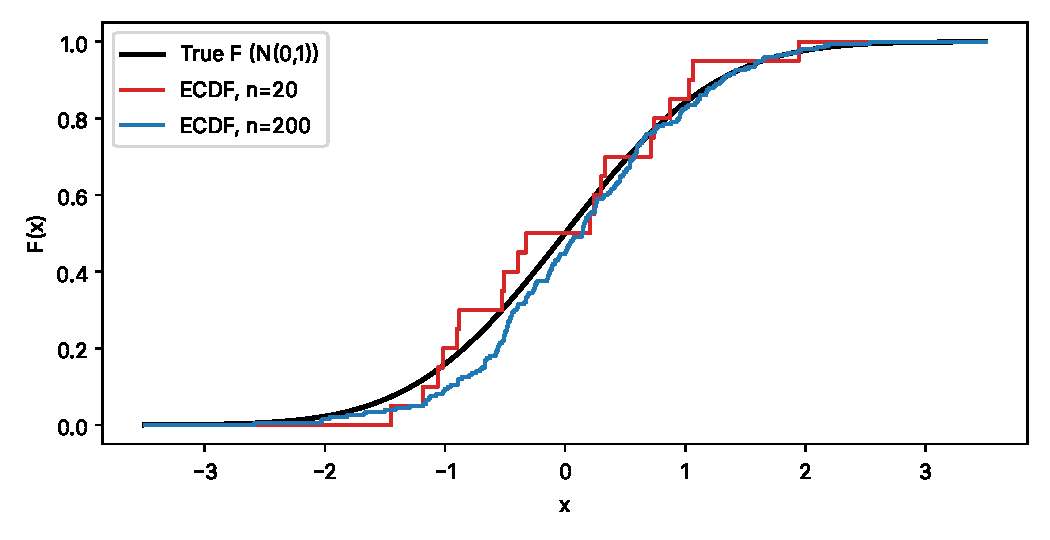
\includegraphics[width=0.85\textwidth]{figures/ecdf.pdf}
\caption{Empirical CDFs of standard normal samples. As $n$ grows, the step function converges uniformly to the true CDF (Glivenko--Cantelli).}
\end{figure}

The output above shows that $\E[\sqrt n D_n]$ stays roughly constant in $n$; this is a numerical confirmation of the $D_n=O_P(n^{-1/2})$ rate and of the Kolmogorov limit distribution (whose mean is $\sqrt{\pi/2}\ln 2\approx0.869$).

\subsection{Inverse Transform and the Probability Integral Transform}

\pycode{code/ch02/c02_3_inverse_transform_pit.py}
\begin{lstlisting}[style=output]
Exponential: mean=0.5002 (theory 0.5), KS p-value=0.964
Cauchy     : median=0.0004 (theory 0), KS p-value=0.964
Poisson    : mean=2.9998, variance=2.9995 (theory 3, 3)
PIT: mean of F(X)=0.4998 (1/2), variance=0.0833 (1/12=0.0833)
\end{lstlisting}

It is no coincidence that the KS\index{kolmogorov smirnov test@Kolmogorov--Smirnov test} $p$-values for the exponential and Cauchy samples are \emph{exactly equal}: both samples were generated from the same vector $U$ through their own $F^{-1}$ and tested with their own $F$. Since $F(F^{-1}(U))=U$, both tests actually test the same sample $U$ against the uniform distribution. This is a direct illustration of the fact that the KS statistic is \emph{distribution-free\index{distribution free statistic@distribution-free statistic}} for continuous $F$ (Theorem~\ref{thm:pit}).

\section{Comments and Notes}

\begin{remark}[Why Is the CDF the Basic Object?]
The distribution $\P_X$ of a random variable\index{random variable@random variable} is a set function on $\B(\R)$ and is hard to work with directly. By the Carathéodory extension theorem, $\P_X$ is \emph{uniquely} determined by its values on the intervals $(-\infty,x]$, that is, by $F_X$. Hence the statement ``two RVs have the same distribution'' is equivalent to ``their CDFs\index{distribution function cdf@distribution function (CDF)} are equal''.
\end{remark}

\begin{remark}[A Density Is Not a Probability]
$f_X(x)$ is not a probability but a probability \emph{density}; it may exceed $1$. For example, for $\text{Uniform}(0,1/2)$, $f_X\equiv2$. Interpretation: for small $h$, $\P(x<X\le x+h)\approx f_X(x)h$.
\end{remark}

\begin{remark}[A Computational Note]
The expression \texttt{[np.mean(samples <= x) for x in x\_grid]} in the first code performs $O(n\cdot|\text{grid}|)$ operations. For large $n$, sorting the sample once and using \texttt{np.searchsorted} gives the ECDF in $O(n\log n)$ time.
\end{remark}

% --- CHAPTER SUMMARY ---
\section{Chapter Summary}
\begin{summary}
\begin{itemize}
  \item A random variable is a measurable function $X:\Omega\to\R$ (Definition~\ref{def:rd}). Its distribution is completely determined by its CDF.
  \item A function is a CDF if and only if it is non-decreasing and right-continuous with limits $0$ and $1$ (Theorem~\ref{thm:cdf-ozellik}). Its jump points are at most countable, and $\P(X=x)=F(x)-F(x^-)$.
  \item The basic equivalence for the quantile function, $F^{-1}(u)\le x\iff u\le F(x)$ (Lemma~\ref{lem:kantil}), yields two results: the inverse transform method (Theorem~\ref{thm:ters-donusum}) and, for continuous $F$, $F(X)\sim\text{Uniform}(0,1)$ (Theorem~\ref{thm:pit}).
  \item Under monotone transformations the density becomes $f_X(g^{-1}(y))\,|(g^{-1})'(y)|$ (Theorem~\ref{thm:donusum}).
  \item By the Glivenko--Cantelli theorem the empirical CDF converges uniformly to the true CDF (Theorem~\ref{thm:glivenko}). The DKW inequality gives this convergence an exponential rate. The bootstrap and the Kolmogorov--Smirnov test rest on this result.
\end{itemize}
\end{summary}
% --- END OF CHAPTER SUMMARY ---

\paragraph{Further reading.} \cite[Chapters~1--2]{casella}, \cite[Chapter~2]{wasserman}; for the empirical CDF\index{empirical distribution function@empirical distribution function}\index{distribution function cdf@distribution function (CDF)} and the DKW\index{dkw inequality@DKW inequality} inequality see \cite[Chapter~7]{wasserman} and \cite[Chapter~19]{vdv}.

\section{Exercises}

\begin{exercise}\label{exr:02-1}
If $X\sim\text{Uniform}(0,1)$, find the distribution of $Y=-2\ln X$ using Theorem~\ref{thm:donusum} and show that it is $\chi^2_2$. Relate this result to Fisher's method of combining $p$-values.
\hfill\hyperref[coz:02-1]{\footnotesize$\rightarrow$\,Solution}
\end{exercise}

\begin{exercise}\label{exr:02-2}
Write the inverse transform algorithm for $F(x)=1-e^{-x^k}$ ($x\ge0$, $k>0$; Weibull) and compare the mean of your generated sample with $\Gamma(1+1/k)$.
\hfill\hyperref[coz:02-2]{\footnotesize$\rightarrow$\,Solution}
\end{exercise}

\begin{exercise}\label{exr:02-3}
Let $X$ and $Y$ be independent with CDFs $F$ and $G$. Find the CDFs of $\max(X,Y)$ and $\min(X,Y)$. Show that for $X_1,\dots,X_n\iid F$ the CDF of $X_{(n)}$ is $F^n$ (this will be used in Chapter~\ref{ch:tamlik}; for general order statistics see Theorem~\ref{thm:sira}).
\hfill\hyperref[coz:02-3]{\footnotesize$\rightarrow$\,Solution}
\end{exercise}

\begin{exercise}\label{exr:02-4}
Using the DKW inequality, find the smallest $n$ such that $\P(D_n>0.02)\le0.05$. From this, construct a $95\%$ confidence \emph{band} for $F$.
\hfill\hyperref[coz:02-4]{\footnotesize$\rightarrow$\,Solution}
\end{exercise}

\end{document}
